\documentclass[letterpaper,9pt]{article}
\usepackage[margin=1.5cm]{geometry}

\usepackage{color}
\usepackage[colorlinks=true]{hyperref}
\usepackage{graphicx}
\usepackage{rotating}

\title{\textbf{Lab3 Protocol}}
\author{Emily Ruppel, Iljoo Baek, Mengwen He}

\begin{document}

\maketitle
\tableofcontents
\newpage

\section{Self-Organization}

\begin{figure}[!h]
	\centering
	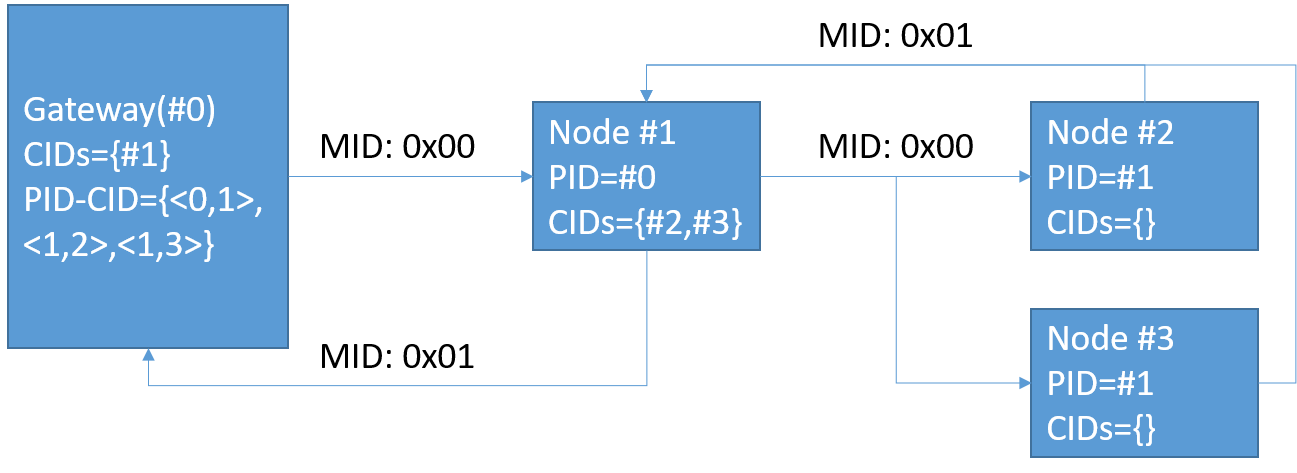
\includegraphics[width=12cm]{./img/selforganization.png}
\end{figure}

\subsection{Gateway}

\subsubsection{TX (G-Thread-1): Message ID 0x00}

\begin{enumerate}
	\item Start (re-)organization at time $t$ (default reorganization interval: 5s configurable)
		%\item Clear children list $\{CID_i$\}
		\item Clear parent-child list $\{<PID,CID>_i\}$
		\item Increase round count $\rho\leftarrow(\rho+1)\%256$
	\item Broadcast an organization message with $\rho$, and node ID $NID$:\\
	\framebox[0.6\textwidth]{Message ID 0x00 [1B], $\rho$ [1B], $NID$ [1B]: e.g. 0x00 0x04 0x00}
	\item \colorbox{yellow}{goto 1}
\end{enumerate}

\subsubsection{RX (G-Thread-2): Message ID 0x01}

\begin{enumerate}
	\item Get and parse the replied organization message (Message ID 0x01)
	\begin{itemize}
		\item received round count $\rho_R$
		\item received parent ID $PID_R$
		\item received parent-child pair $<PID,CID>_R$	
	\end{itemize}
		\item If $\rho_R \neq \rho$ or $PID_R \neq NID$, then \colorbox{yellow}{goto 1}
		%\item If $PID_R = <PID,CID>_R::PID$, then add $<PID,CID>_R::CID$ to $\{CID_i\}$
		\item If $PID_R = <PID,CID>_R::PID$, then reply an acknowledge message with $\rho$, $NID$:\\
		\framebox[0.8\textwidth]{Message ID 0x02 [1B], $\rho$ [1B], $NID$ [1B]: e.g. 0x02 0x04 0x00}
		\item Add $<PID,CID>_R$ to $\{<PID,CID>_i\}$ and refresh the neighbor list of $<PID,CID>_R::PID$ node.
	\item \colorbox{yellow}{goto 1}	
\end{enumerate}

\subsection{Communication Node}

\subsubsection{RX (N-Thread-1): Message ID 0x00}

\begin{enumerate}
	\item Get and parse the organization message (Message ID 0x00):
	\begin{itemize}
		\item received round count $\rho_R$
		\item received note ID $NID_R$
		\item RSSI level $\Phi$
	\end{itemize}
	\item If $\Phi<\Phi^*$ ($\Phi^*$ is the minimum required RSSI to build a reliable wireless connection), then \colorbox{yellow}{goto 1}
	\item If its own round count $\rho=\rho_R$, then \colorbox{yellow}{goto 1}
		%\item Clear children list $\{CID_i\}$
		\item Set round count: $\rho=\rho_R$
		\item Set parent ID: $PID=NID_R$
		\item Reply an acknowledge message with $\rho$, $PID$, and $NID$:\\
		\framebox[0.8\textwidth]{Message ID 0x01 [1B], $\rho$ [1B], $PID$ [1B], $<PID,NID>$ [2B]: e.g. 0x01 0x04 0x01 0x01 0x02}
	\item \colorbox{yellow}{goto 1}
\end{enumerate}

\subsubsection{RX (N-Thread-1): Message ID 0x01}

\begin{enumerate}
	\item Get and parse the replied organization message (Message ID 0x01)
	\begin{itemize}
		\item received round count $\rho_R$
		\item received parent ID $PID_R$
		\item received parent-child pair $<PID,CID>_R$
	\end{itemize}
		\item If $\rho_R \neq \rho$ or $PID_R \neq NID$, then \colorbox{yellow}{goto 1}
		%\item If $PID_R = <PID,CID>_R::PID$, then add $<PID,CID>_R::CID$ to $\{CID_i\}$
		\item If $PID_R = <PID,CID>_R::PID$, then reply an acknowledge message with $\rho$, $NID$:\\
		\framebox[0.8\textwidth]{Message ID 0x02 [1B], $\rho$ [1B], $NID$ [1B]: e.g. 0x02 0x04 0x01}
		\item Relay an acknowledge message with $\rho$, $PID$, and  $<PID,CID>_R$:\\
		\framebox[0.8\textwidth]{Message ID 0x01 [1B], $\rho$ [1B], $PID$ [1B], $<PID,CID>_R$ [2B]: e.g. 0x01 0x04 0x00 0x01 0x02}
	\item \colorbox{yellow}{goto 1}	
\end{enumerate}

\subsubsection{RX (N-Thread-1): Message ID 0x02}

\begin{enumerate}
	\item Get and parse the replied organization acknowledge message (Message ID 0x02)
	\begin{itemize}
		\item received round count $\rho_R$
		\item received parent ID $PID_R$
	\end{itemize}
	\item If $\rho_R \neq \rho$ or $PID_R \neq PID$, then \colorbox{yellow}{goto 1}
	%\item If $PID_R = <PID,CID>_R::PID$, then add $<PID,CID>_R::CID$ to $\{CID_i\}$
		\item Broadcast an organization message with $\rho$, and $NID$:\\
	\framebox[0.6\textwidth]{Message ID 0x00 [1B], $\rho$ [1B], $NID$ [1B]: e.g. 0x00 0x04 0x01}
	\item \colorbox{yellow}{goto 1}	
\end{enumerate}

\newpage
\section{Upload Light Values}

\begin{figure}[!h]
	\centering
	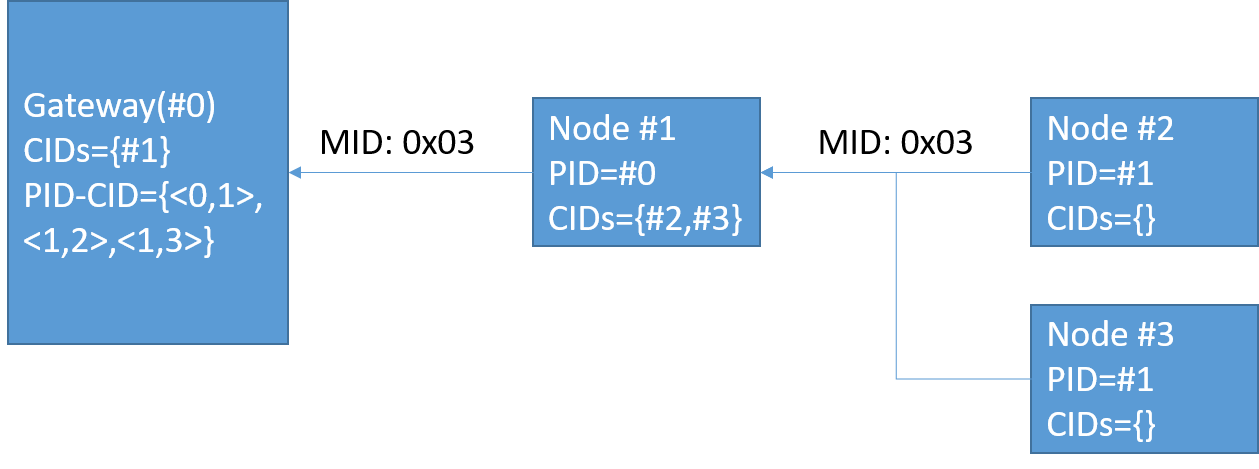
\includegraphics[width=12cm]{./img/lightvalue.png}
\end{figure}

\subsection{Gateway}

\subsubsection{RX (G-Thread-2): Message ID 0x03}

\begin{enumerate}
	\item Get and parse the light value message (Message ID 0x03)
	\begin{itemize}
		\item received round count $\rho_R$
		\item received parent ID $PID_R$
		\item received node ID $NID_R$
		\item received timestamp $Sec_R$, $NSec_R$
		\item received light value $L_R$
	\end{itemize}
		\item If $\rho_R \neq \rho$ or $PID_R \neq NID$, then \colorbox{yellow}{goto 1}
		\item Display light value ``$Sec_R$ s + $NSec_R$ nsec : $NID_R$'s light value is $L_R$"
	\item \colorbox{yellow}{goto 1}
\end{enumerate}

\subsection{Communication Node}

\subsubsection{RX (N-Thread-1): Message ID 0x03}

\begin{enumerate}
	\item Get and parse the light value message (Message ID 0x03)
	\begin{itemize}
		\item received round count $\rho_R$
		\item received parent ID $PID_R$
		\item received node ID $NID_R$
		\item received timestamp $Sec_R$, $NSec_R$
		\item received light value $L_R$
	\end{itemize}
		\item If $\rho_R \neq \rho$ or $PID_R \neq NID$, then \colorbox{yellow}{goto 1}
		\item Relay light value message with $\rho$, $PID$, $NID$, timestamp $Sec_R+NSec_R$, and $L_t$ to parent:\\
		\framebox[0.85\textwidth]{Message ID 0x03 [1B], $\rho$[1B], $PID$ [1B], $NID_R$ [1B], $Sec_R$ [4B], $NSec_R$ [4B], $L_R$ [2B]}\\
		\framebox[0.85\textwidth]{e.g. 0x03 0x04 0x00 0x02 0x19 0x90 0x11 0x23 0x19 0x88 0x10 0x25 0x11 0x23}
	\item \colorbox{yellow}{goto 1}
\end{enumerate}

\subsubsection{TX (N-Thread-2): Message ID 0x03}

\begin{enumerate}
	\item Sample start at time $t$ (sample rate is controlled by $dt$ ms and is configurable via gateway)
	\item Get light value $L_t$
		\item Send light value message with $\rho$, $PID$, $NID$, timestamp $Sec+NSec$, and $L_t$ to parent:\\
		\framebox[0.85\textwidth]{Message ID 0x03 [1B], $\rho$[1B], $PID$ [1B], $NID$ [1B], $Sec$ [4B], $NSec$ [4B], $L_t$ [2B]}\\
		\framebox[0.85\textwidth]{e.g. 0x03 0x04 0x01 0x02 0x19 0x90 0x11 0x23 0x19 0x88 0x10 0x25 0x11 0x23}
	\item \colorbox{yellow}{goto 1}
\end{enumerate}

\newpage
\section{Configure Sample Rate [This can be done via broadcast]}

\begin{figure}[!h]
	\centering
	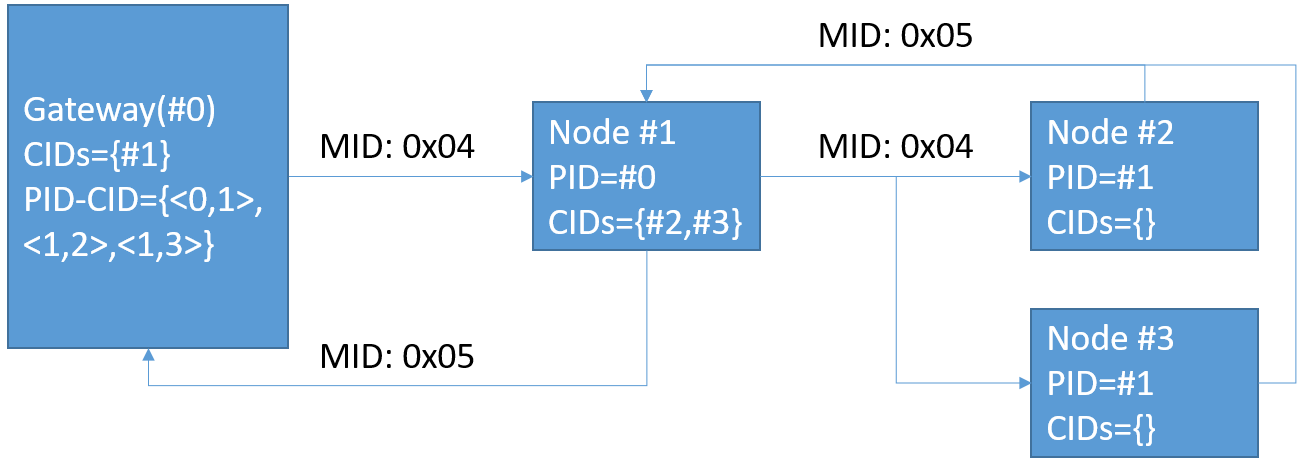
\includegraphics[width=12cm]{./img/samplerate.png}
\end{figure}

\subsection{Gateway}

\subsubsection{TX2 (G-Thread-3): Message ID 0x04}

\begin{enumerate}
	\item Give a new sample rate $dt$
		\item Broadcast a sample rate message with $\rho$, $NID$, and $dt$ (ms):\\
		\framebox[0.85\textwidth]{Message ID 0x04 [1B], $\rho$[1B], $NID$ [1B], $dt$ [4B]: e.g. 0x04 0x04 0x00 0x19 0x90 0x11 0x23}
\end{enumerate}

\subsubsection{RX (G-Thread-2): Message ID 0x05}

\begin{enumerate}
	\item Get and parse the sample rate update message (Message ID 0x05)
	\begin{itemize}
		\item received round count $\rho_R$
		\item received parent ID $PID_R$
		\item received node ID $NID_R$
		\item received sample rate $dt_R$
	\end{itemize}
		\item If $\rho_R \neq \rho$ or $PID_R \neq NID$, then \colorbox{yellow}{goto 1}
		\item Display sample rate update info ``$NID_R$'s sample rate changes to $dt_R$"
	\item \colorbox{yellow}{goto 1}
\end{enumerate}

\subsection{Communication Node}

\subsubsection{RX (N-Thread-1): Message ID 0x04}

\begin{enumerate}
	\item Get and parse the sample rate message (Message ID 0x04)
	\begin{itemize}
		\item received round count $\rho_R$
		\item received parent ID $PID_R$
		\item received sample rate $dt_R$
	\end{itemize}
		\item If $\rho_R \neq \rho$ or $PID_R \neq PID$, then \colorbox{yellow}{goto 1} [No need to check $PID_R$ with $PID$ if using broadcast]
		\item Set $dt=dt_R$
		\item Reply a sample rate update message with $\rho$, $PID$, $NID$, and $dt$ (ms):\\
		\framebox[0.9\textwidth]{Message ID 0x05 [1B], $\rho$[1B], $PID$ [1B], $NID$ [1B], $dt$ [4B]: e.g. 0x05 0x04 0x01 0x02 0x19 0x90 0x11 0x23}
		\item Relay a sample rate message with $\rho$, $NID$, and $dt$ (ms):\\
		\framebox[0.85\textwidth]{Message ID 0x04 [1B], $\rho$[1B], $NID$ [1B], $dt$ [4B]: e.g. 0x04 0x04 0x01 0x19 0x90 0x11 0x23}
	\item \colorbox{yellow}{goto 1}
\end{enumerate}

\subsubsection{RX (N-Thread-1): Message ID 0x05}

\begin{enumerate}
	\item Get and parse the sample rate update message (Message ID 0x05)
	\begin{itemize}
		\item received round count $\rho_R$
		\item received parent ID $PID_R$
		\item received node ID $NID_R$
		\item received light value $dt_R$
	\end{itemize}
		\item If $\rho_R \neq \rho$ or $PID_R \neq NID$, then \colorbox{yellow}{goto 1}
		\item Relay sample rate update message with $\rho$, $PID$, $NID_R$, and $dt_R$ to parent:\\
		\framebox[0.92\textwidth]{Message ID 0x05 [1B], $\rho$[1B], $PID$ [1B], $NID_R$ [1B], $dt_R$ [4B]: e.g. 0x05 0x04 0x00 0x02 0x19 0x90 0x11 0x23}
	\item \colorbox{yellow}{goto 1}
\end{enumerate}

\newpage
\section{Message Protocol}

\begin{center}
	\rotatebox{90}{
		\small
		\begin{tabular}{|c|l|c|c|c|c|}
			\hline
			\textbf{ID}	&	\textbf{Code}	&	\textbf{Length}	&	\textbf{Note} & \textbf{Directions} & \textbf{Need Relay}	\\
			\hline
			\hline
			0x00		&	0x00 [1], $\rho$ [1], $NID$ [1]	& 3	&	Organization Message	&	Parent $\rightarrow$ Child & Y	\\
			\hline
			0x01		&	0x01 [1], $\rho$ [1], $PID$ [1], $CID$ [2]	&	4	&	Organization Message Reply	& Child $\rightarrow$ Parent & Y	\\
			\hline
			0x02		&	0x02 [1], $\rho$ [1], $NID$ [1]	& 3	&	Organization Message Reply Ack	&	Parent $\rightarrow$ Child & N	\\
			\hline
			\hline
			0x03		&	0x03 [1], $\rho$ [1], $PID$ [1], $PID_{(R)}$ [1], $NID_{(R)}$ [1], $Sec_{(R)}$ [4], $NSec_{(R)}$ [4], $L_{t/R}$ [2]	&	15	&	Light Value Message & Child $\rightarrow$ Parent & Y \\
			\hline
			\hline
			0x04		&	0x04 [1], $\rho$ [1], $NID$ [1], $dt$ [4] & 7 & Sample Rate Message & Parent $\rightarrow$ Child & Y \\
			\hline
			0x05		&	0x05 [1], $\rho$ [1], $PID$ [1], $NID_{(R)}$ [1], $dt_{(R)}$ [4] & 8 & Sample Rate Updated Message & Child $\rightarrow$ Parent & Y \\
			\hline		
		\end{tabular}
	}
\end{center}


\end{document}